%!TEX root = mainfile.tex

\section{Ground Based versus Space Based Telescopes} % (fold)
\label{sec:ground_based_versus_space_based_telescopes}
	Ground based telescopes and space based telescopes have distinct advantages and disadvantages over one another and these must be considered when deciding which telescope or telescopes to use as part of the final observing strategy. This section looks at these advantages and disadvantages whilst also looking to the future for new developments which could prove useful to the overall project.

	Ground based telescopes are seeing limited which is a resolving limitation due to distortion caused by the atmosphere. Light is scattered by the atmosphere and so detecting a source by these telescopes can be difficult. This is discussed further in Section~\ref{sub:astronomical_seeing}. There is also the limitation of considerably more background light, compared to what is measured by space telescopes. To minimise these limitations, ground based telescopes are usually located at high altitude at locations such as Mauna Kea, Hawaii or Cerro Paranal, Chile. The main advantage of ground based telescopes however is that they can be built to very large sizes with telescopes with a primary diameter of around \SI{30}{\metre} on the periphery. This cannot be achieved by space telescopes as the cost of transport to space would be very large and the telescope may well be damaged during this transportation. This also provides the ground based telescopes with very large fields of view meaning they can see more of the sky in a single observation. Importantly, they are also much cheaper to build and maintain.

	Space based telescopes are diffraction limited, i.e.\ the main limitation is whether the angular resolution of the telescope can resolve the object being observed. Light arriving from the source is diffracted at the telescopes aperture spreading out the light. This subtends to an angle and becomes the minimum angle that the telescope can resolve. This is important as light from other sources in the sky may almost overlap and so this diffraction limited angle gives the angle in the sky which can be resolved. Thus if the diffraction angle is small, the better the resolving power of the telescope. Should two sources fall within this diffraction angle when looking into the sky, the telescope will not be able to resolve the two objects and so one cannot be distinguished from another. The angular resolution of the telescope can be calculated according to the Rayleigh criterion below where $\lambda$ is the wavelength of the incoming photon and $D$ is the primary mirror diameter of the telescope
	\begin{align}
		\Delta\theta= \frac{(1.22 \lambda)}{D}
	\end{align}
	This also shows that the larger the diameter, the smaller the diffraction angle will be and so the better the telescope will be at resolving sources. This gives space based telescopes a distinct advantage over ground based telescopes as the seeing limitation of ground based telescopes often means that the diffraction angle is superseded. The source blurred by the atmosphere has a much greater spreading of light and so the smallest angle that it is possible to resolve is therefore much larger meaning the telescope will not be as effective when looking at distant sources. Other advantages of space based telescopes include receiving considerably less background light and that they can be operated for longer time periods during the day whereas ground based telescopes cannot be used for observations during the daytime or in adverse weather conditions such as a cloudy sky.

	The main disadvantage of space based telescope is that they are vastly more expensive to build and maintain and must also be transported into space. This is usually done with the aid of a rocket and so the cost of achieving this can be considerable. The telescope may also be damaged during this transportation and so this limits the size of the telescope as a smaller size will mean a smaller chance of being damaged. The James Webb Space Telescope scheduled for launch in 2018 consists of a 6.5\,metre primary mirror made up of multiple mirrors that will unfold once it is in space. Despite this folding up of the telescope, the primary mirror size is still small relative to some ground based ones currently in use such as the VLT (primary mirror of 8.2\,metres) and is considerably smaller than some proposed for the future such as the EELT (primary mirror 39.3\,metres).

	\subsection{Astronomical Seeing} % (fold)
	\label{sub:astronomical_seeing}
		Plane waves from a source being observed are distorted by the Earth's atmosphere and so upon reaching a telescope within the atmosphere are slightly perturbed and the image formed, blurred. This effect is contributed to by numerous layers where different temperatures or the interaction of different wind speed causes this effect with ``Seeing'' the term used to describe the total distortion of the wavefront\cite[p.~188]{Diffraction_Limited_Imaging_Saha}. This effect is shown below in Figure~\ref{fig:Seeing} where a turbulent layer of the atmosphere causes a change in the shape of the wavefront. This turbulence is caused by micro-thermal fluctuations which can be caused by a variety of reasons such as friction encountered by air flow at the Earth's surface or differential heating of the Earth's surface\cite[p.~161]{Diffraction_Limited_Imaging_Saha}.
		\begin{figure}[!htbp]
			\centering
			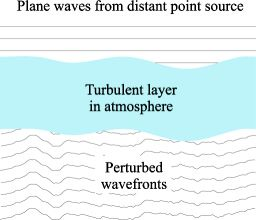
\includegraphics[width=0.4\textwidth]{../Images/Seeing.png}
			\caption{The perturbation of a wavefront due to the atmosphere\cite{Seeing}\label{fig:Seeing}}
		\end{figure}

		Whilst the resolving power of a telescope is generally largely dependent on its diameter, this seeing limitation becomes the major source of error when resolving a point source from within the Earth's atmosphere. This is consequently the main limitation for ground based telescopes which are therefore known as being seeing limited. A point spread function (PSF) imaged in these circumstances produces what is known as a seeing disc due to the atmospheric turbulence and the most common measurement used to describe this effect is the full width at half maximum (FWHM), shown below in Figure~\ref{fig:FWHM} where a peak shape is produced by this overall blurring of the source. When measuring the flux arriving at the CCD from a particular source, an area of radius four times the FWHM is recorded over and so a larger value of FWHM also increases the integration time required to observe the source. A derivation of how to calculate the FWHM is given in Section~\ref{sub:full_width_at_half_maximum}.
		\begin{figure}[!htbp]
			\centering
			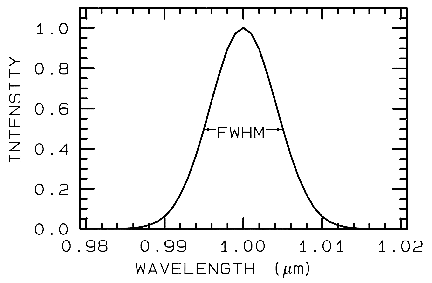
\includegraphics[width=0.5\textwidth]{../Images/FWHM.png}
			\caption{A peak produced by the blurring of a point source}\label{fig:FWHM}
		\end{figure}
	% subsection astronomical_seeing (end)

	\subsection{The Future of Ground Based Telescopes} % (fold)
	\label{sub:the_future_of_ground_based_telescopes}
		The main disadvantage of ground based telescopes compared to space based telescopes is the poorer resolution due to the distortion caused by the atmosphere or astronomical seeing. The introduction of adaptive optics however, should help resolve this issue and allow ground based telescopes to be only diffraction limited similar to space based ones. This, combined with the large diameter mirrors currently in the pipeline such as for the European Extremely Large Telescope (E-ELT), a primary mirror of 39.3\,metres, and the Giant Magellan Telescope (GMT), a primary mirror of 25\,metres, ensure ground based telescopes hold a place in the future of space observation, even if just to compliment space based ones. The larger mirrors ensure a greater light collecting power, receiving more photons for the source being observed and so significantly reducing the observing time required. These large diameter mirrors are currently only possible for ground based telescopes and so provide them with a distinct advantage over space based ones.

		\subsubsection{Adaptive Optics} % (fold)
		\label{ssub:adaptive_optics}
			As described earlier in astronomical seeing, light passing through the atmosphere from a source, such as a distant galaxy, is perturbed due to atmospheric turbulence and so the images produced by ground based telescopes are blurred. Adaptive optics works by first sensing the wavefront perturbations and then counteracting this blurring in real time thus enabling the telescopes to hold a much larger resolving power. This is usually done with light from a guide star although as sufficiently bright natural guide stars are not readily available, it is possible to use a laser guide stars produced by the observatory. This system will be used on future ground based telescopes ensuring they are no longer limited by the ability to resolve a source. An example of how this is set up, as on the Subaru Telescope, is shown below in Figure~\ref{fig:AdaptiveOptics}.
			\begin{figure}[!htbp]
				\centering
				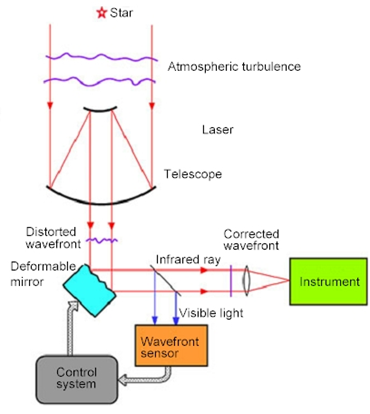
\includegraphics[width=0.5\textwidth]{../Images/AdaptiveOptics.png}
				\caption{A schematic of an adaptive optics system\cite{Adaptive}}\label{fig:AdaptiveOptics}
			\end{figure}

			The wavefront sensor (WFS) measures the distortions in the incoming wavefront of light. This then provides the measured information to an actuator control computer identified in Figure~\ref{fig:AdaptiveOptics} as the control system. This then adjusts the shape of the adjustable mirror to effectively correct the wavefront reaching the telescope\cite{Diffraction_Limited_Imaging_Saha}.  The wavefront sensor can measure the distortions introduced into the wavefront on the timescale of a few milliseconds with the information then computed and the shape of the mirror adjusted accordingly. The correction process should therefore be completed in a time similar to the time between the changes of the wavefront thus ensuring the distortion is compensated for.
		% subsubsection adaptive_optics (end)
	% subsection the_future_of_ground_based_telescopes (end)
% section ground_based_versus_space_based_telescopes (end)
